\documentclass{beamer}
\usepackage{luatexja}
\usepackage{tikz}
\usepackage[mark=o]{dynkin-diagrams}
\usetikzlibrary{calc}
\usetheme{Luebeck}
\usecolortheme{seahorse}
\usefonttheme{structurebold,serif}
\setbeamertemplate{navigation symbols}{\usebeamerfont{footline}\insertframenumber/\inserttotalframenumber}

\title{平面の敷き詰めとルート系}
\author{宇佐見 公輔}
\date{2020年06月28日 日曜数学会}
\begin{document}
\maketitle

\begin{frame}
    \frametitle{自己紹介}

    職業:プログラマ / 趣味:数学

    \bigskip

    最近の活動(登壇・ブログ・Twitter):
    \begin{itemize}
        \item 四元数のはなし(2020年5月 / 関西日曜数学友の会)
        \item はじめて学ぶリー環 ノート(2020年4月〜 / Twitter)
        \item Ising 模型 ノート(2020年3月〜4月 / Twitter)
        \item Onsager 代数の話(2020年3月 / 京都某所)
        \item はじめて学ぶリー群 ノート(2020年1月〜3月 / Twitter)
        \item リー代数と結合法則(2019年12月 / Advent Calendar)
        \item 回転群のはなし(2019年11月 / 関西日曜数学友の会)
        \item 行列の指数関数(2019年10月 / 関西数学徒のつどい)
        \item リー代数の計算の楽しみ(2019年10月 / マスパーティ)
    \end{itemize}
\end{frame}

\begin{frame}
    \frametitle{平面の敷き詰め問題}

    \begin{block}{問題}
        三角形を辺で折り返す操作を繰り返すとき、
        互いに重ならずに、すき間なく平面を敷き詰めることができる条件は?
    \end{block}

    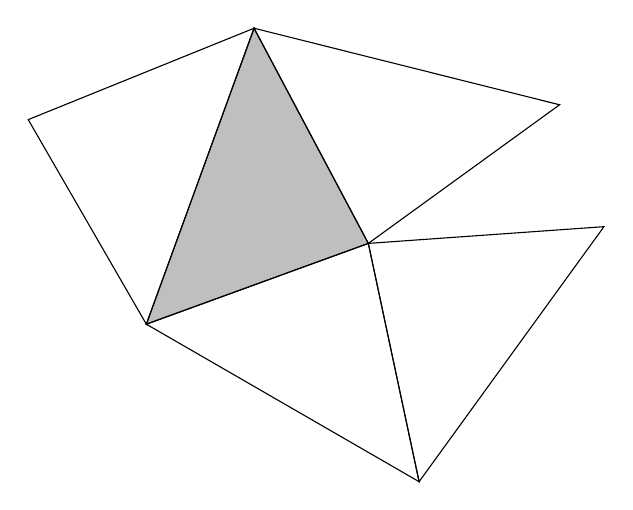
\begin{tikzpicture}
        \coordinate (A) at (0,0);
        \coordinate (B) at (20:3);
        \coordinate (C) at (70:4);
        \filldraw[fill=lightgray] (A) -- (B) -- (C) -- cycle;
        \coordinate (AB) at ($ (A)!(C)!(B) $);
        \coordinate (C') at ($ (C)!2!(AB) $);
        \draw (A) -- (B) -- (C') -- cycle;
        \coordinate (AC) at ($ (A)!(B)!(C) $);
        \coordinate (B') at ($ (B)!2!(AC) $);
        \draw (A) -- (B') -- (C) -- cycle;
        \coordinate (BC) at ($ (B)!(A)!(C) $);
        \coordinate (A') at ($ (A)!2!(BC) $);
        \draw (A') -- (B) -- (C) -- cycle;
        \coordinate (BC') at ($ (B)!(A)!(C') $);
        \coordinate (A'') at ($ (A)!2!(BC') $);
        \draw (A'') -- (B) -- (C') -- cycle;
    \end{tikzpicture}
\end{frame}

\begin{frame}
    \frametitle{ヒント}

    三角形の各頂点に \(\mathrm{A}\)、\(\mathrm{B}\)、\(\mathrm{C}\) と名前をつけておきます。

    \bigskip

    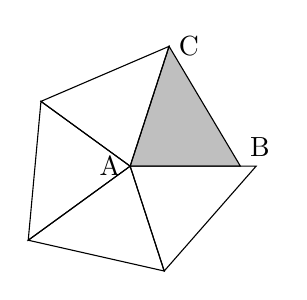
\begin{tikzpicture}
        \coordinate (A) at (0,0);
        \coordinate (B) at (0:1.4);
        \coordinate (C) at (360/5:1.6);
        \node (AA) at (A) [left] {A};
        \node (BB) at (B) [above right] {B};
        \node (CC) at (C) [right] {C};
        \filldraw[fill=lightgray] (A) -- (B) -- (C) -- cycle;
        \draw (A) -- (C) -- (360/5*2:1.4) -- cycle;
        \draw (A) -- (360/5*2:1.4) -- (360/5*3:1.6) -- cycle;
        \draw (A) -- (360/5*3:1.6) -- (360/5*4:1.4) -- cycle;
        \draw (A) -- (360/5*4:1.4) -- (0:1.6) -- cycle;
    \end{tikzpicture}

    \bigskip

    頂点 \(\mathrm{A}\) のまわりには、頂点 \(\mathrm{B}\)、\(\mathrm{C}\) は来ません。
    よって、\(\angle \mathrm{A}\) の整数倍が \(360^\circ \) ちょうどになる必要があります。
    (\(\angle \mathrm{B}\)、\(\angle \mathrm{C}\) も同様)

    \bigskip

    頂点 \(\mathrm{A}\) のまわりに集まる角が奇数個の場合、辺 \(\mathrm{AB}\) と辺 \(\mathrm{AC}\) が重なるため、
    \(\mathrm{AB} = \mathrm{AC}\) である必要があり、 \(\angle \mathrm{B} = \angle \mathrm{C}\) となります。
    (\(\mathrm{B}\)、\(\mathrm{C}\) についても同様)
\end{frame}

\begin{frame}
    \frametitle{平面の敷き詰め問題の解}

    先ほどのヒントがあれば、あとは場合分けして解くことができます。

    \bigskip

    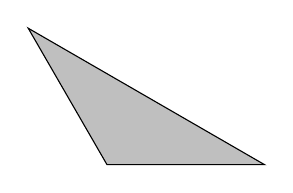
\begin{tikzpicture}
        \filldraw[fill=lightgray] (0,0) -- (0:2) -- (120:2) -- cycle;
    \end{tikzpicture}
    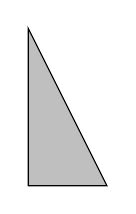
\begin{tikzpicture}
        \filldraw[fill=lightgray] (0,0) -- (0:1) -- (90:2) -- cycle;
    \end{tikzpicture}
    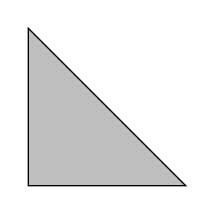
\begin{tikzpicture}
        \filldraw[fill=lightgray] (0,0) -- (0:2) -- (90:2) -- cycle;
    \end{tikzpicture}
    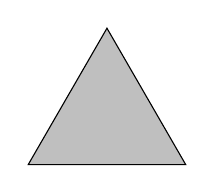
\begin{tikzpicture}
        \filldraw[fill=lightgray] (0,0) -- (0:2) -- (60:2) -- cycle;
    \end{tikzpicture}
\end{frame}

\begin{frame}
    \frametitle{リー代数}

    話は変わって・・・

    \bigskip

    \begin{block}{リー代数}
        ベクトル空間 = 「加法」と「スカラー倍」

        リー代数 = ベクトル空間 + 第3の演算「ブラケット積」
    \end{block}

    ブラケット積が満たすべき条件
    \begin{enumerate}
        \item \([ax + by, z] = a[x, z] + b[y, z]\), \\
              \([z, ax + by] = a[z, x] + b[z, y]\)(双線型性)
        \item \([x, x] = 0\) (\(\implies [x, y] = - [y, x]\))(交代性)
        \item \([x, [y, z]] + [y, [z, x]] + [z, [x, y]] = 0\)(Jacobi identity)
    \end{enumerate}
\end{frame}

\begin{frame}
    \frametitle{リー代数はどこで出てくるか}

    リー代数は、代表的なものとしては以下のようなところで出てきます。

    \begin{block}{リー群とリー代数}
        リー群(群構造を持つ微分多様体)の接ベクトル空間がリー代数になります。
    \end{block}

    \begin{block}{数理物理モデルとリー代数}
        例えば、強磁性体のモデルであるイジングモデルは、厳密解をリー代数を使って求めることができます。
    \end{block}
\end{frame}

\begin{frame}
    \frametitle{ディンキン図形}

    実のところ僕は、リー群や数理物理とは無関係なところから、リー代数に興味を持ちました。
    そのきっかけがディンキン図形。

    \begin{example}[ディンキン図形]
        \scalebox{3}{
            \dynkin{A}{3}
        }
        \scalebox{3}{
            \dynkin{C}{5}
        }
        \scalebox{3}{
            \dynkin{D}{4}
        }
        \scalebox{3}{
            \dynkin{E}{6}
        }
        \scalebox{3}{
            \dynkin{F}{4}
        }
        \scalebox{3}{
            \dynkin{G}{2}
        }
    \end{example}
\end{frame}

\begin{frame}
    \frametitle{ディンキン図形の種類}

    ディンキン図形を初めて見かけたとき、「これはなんだろう?」と不思議に思ったのが第一印象。
    「これって数学・・・?」

    \bigskip

    その後、有限次元複素単純リー代数の分類がこの図形で行われることを知り、
    リー代数の理論に興味を持ちました。

    \bigskip

    \begin{block}{ディンキン図形の種類(有限次元複素単純リー代数の分類)}
        \begin{itemize}
            \item \(A_n\) (\(n = 1,2,3,4,5,\dots\))
            \item \(B_n\) (\(n = 2,3,4,5,\dots\))
            \item \(C_n\) (\(n = 3,4,5,\dots\))
            \item \(D_n\) (\(n = 4,5,\dots\))
            \item \(E_6\), \(E_7\), \(E_8\), \(F_4\), \(G_2\)
        \end{itemize}
    \end{block}
\end{frame}

\begin{frame}
    \frametitle{ルート系}

    ルート系は、ユークリッド空間内のベクトルの集合で、ある公理を満たすものです。

    \bigskip

    ディンキン図形は、ルート系を特定のルールによって図で表現したものです。
    ルート系とディンキン図形は1対1対応しています。

    \bigskip

    2次元のルート系は、\(A_2\), \(B_2\), \(G_2\) があります。

    \bigskip

    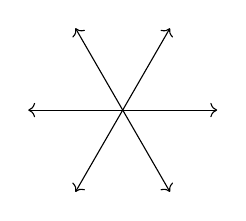
\begin{tikzpicture}
        \draw[->] (0,0) -- (0:1.2);
        \draw[->] (0,0) -- (60:1.2);
        \draw[->] (0,0) -- (120:1.2);
        \draw[->] (0,0) -- (180:1.2);
        \draw[->] (0,0) -- (240:1.2);
        \draw[->] (0,0) -- (300:1.2);
    \end{tikzpicture}
    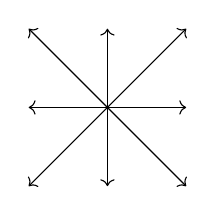
\begin{tikzpicture}
        \draw[->] (0,0) -- (1,0);
        \draw[->] (0,0) -- (1,1);
        \draw[->] (0,0) -- (0,1);
        \draw[->] (0,0) -- (-1,1);
        \draw[->] (0,0) -- (-1,0);
        \draw[->] (0,0) -- (-1,-1);
        \draw[->] (0,0) -- (0,-1);
        \draw[->] (0,0) -- (1,-1);
    \end{tikzpicture}
    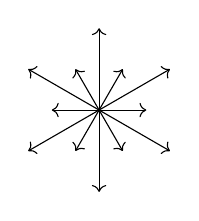
\begin{tikzpicture}
        \draw[->] (0,0) -- (0:0.6);
        \draw[->] (0,0) -- ($ (0:0.6) + (60:0.6) $);
        \draw[->] (0,0) -- (60:0.6);
        \draw[->] (0,0) -- ($ (60:0.6) + (120:0.6) $);
        \draw[->] (0,0) -- (120:0.6);
        \draw[->] (0,0) -- ($ (120:0.6) + (180:0.6) $);
        \draw[->] (0,0) -- (180:0.6);
        \draw[->] (0,0) -- ($ (180:0.6) + (240:0.6) $);
        \draw[->] (0,0) -- (240:0.6);
        \draw[->] (0,0) -- ($ (240:0.6) + (300:0.6) $);
        \draw[->] (0,0) -- (300:0.6);
        \draw[->] (0,0) -- ($ (300:0.6) + (0:0.6) $);
    \end{tikzpicture}
\end{frame}

\begin{frame}
    \frametitle{なんか似てる}

    平面の敷き詰め問題の解

    \bigskip

    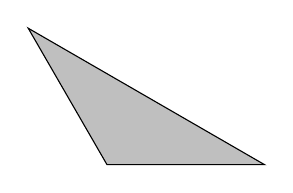
\begin{tikzpicture}
        \filldraw[fill=lightgray] (0,0) -- (0:2) -- (120:2) -- cycle;
    \end{tikzpicture}
    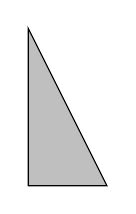
\begin{tikzpicture}
        \filldraw[fill=lightgray] (0,0) -- (0:1) -- (90:2) -- cycle;
    \end{tikzpicture}
    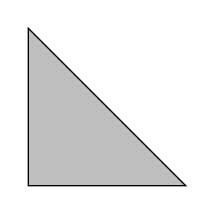
\begin{tikzpicture}
        \filldraw[fill=lightgray] (0,0) -- (0:2) -- (90:2) -- cycle;
    \end{tikzpicture}
    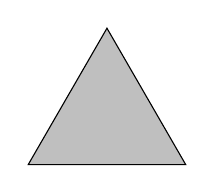
\begin{tikzpicture}
        \filldraw[fill=lightgray] (0,0) -- (0:2) -- (60:2) -- cycle;
    \end{tikzpicture}

    \bigskip

    ルート系

    \bigskip

    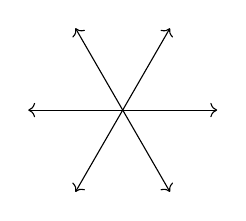
\begin{tikzpicture}
        \draw[->] (0,0) -- (0:1.2);
        \draw[->] (0,0) -- (60:1.2);
        \draw[->] (0,0) -- (120:1.2);
        \draw[->] (0,0) -- (180:1.2);
        \draw[->] (0,0) -- (240:1.2);
        \draw[->] (0,0) -- (300:1.2);
    \end{tikzpicture}
    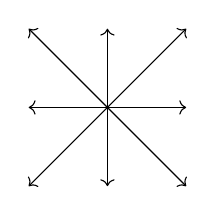
\begin{tikzpicture}
        \draw[->] (0,0) -- (1,0);
        \draw[->] (0,0) -- (1,1);
        \draw[->] (0,0) -- (0,1);
        \draw[->] (0,0) -- (-1,1);
        \draw[->] (0,0) -- (-1,0);
        \draw[->] (0,0) -- (-1,-1);
        \draw[->] (0,0) -- (0,-1);
        \draw[->] (0,0) -- (1,-1);
    \end{tikzpicture}
    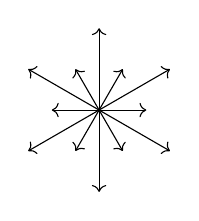
\begin{tikzpicture}
        \draw[->] (0,0) -- (0:0.6);
        \draw[->] (0,0) -- ($ (0:0.6) + (60:0.6) $);
        \draw[->] (0,0) -- (60:0.6);
        \draw[->] (0,0) -- ($ (60:0.6) + (120:0.6) $);
        \draw[->] (0,0) -- (120:0.6);
        \draw[->] (0,0) -- ($ (120:0.6) + (180:0.6) $);
        \draw[->] (0,0) -- (180:0.6);
        \draw[->] (0,0) -- ($ (180:0.6) + (240:0.6) $);
        \draw[->] (0,0) -- (240:0.6);
        \draw[->] (0,0) -- ($ (240:0.6) + (300:0.6) $);
        \draw[->] (0,0) -- (300:0.6);
        \draw[->] (0,0) -- ($ (300:0.6) + (0:0.6) $);
    \end{tikzpicture}
\end{frame}

\begin{frame}
    \frametitle{平面の敷き詰めとルート系}

    実は対応関係があります。(注:\(G_2\) は例外的に2つと対応している)

    \bigskip

    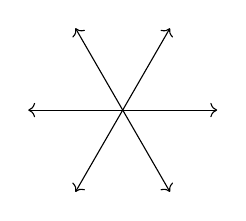
\begin{tikzpicture}
        \draw[->] (0,0) -- (0:1.2);
        \draw[->] (0,0) -- (60:1.2);
        \draw[->] (0,0) -- (120:1.2);
        \draw[->] (0,0) -- (180:1.2);
        \draw[->] (0,0) -- (240:1.2);
        \draw[->] (0,0) -- (300:1.2);
    \end{tikzpicture}
    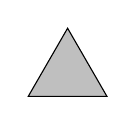
\begin{tikzpicture}
        \filldraw[fill=lightgray] (0,0) -- (0:1) -- (60:1) -- cycle;
    \end{tikzpicture}

    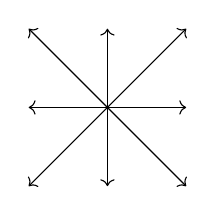
\begin{tikzpicture}
        \draw[->] (0,0) -- (1,0);
        \draw[->] (0,0) -- (1,1);
        \draw[->] (0,0) -- (0,1);
        \draw[->] (0,0) -- (-1,1);
        \draw[->] (0,0) -- (-1,0);
        \draw[->] (0,0) -- (-1,-1);
        \draw[->] (0,0) -- (0,-1);
        \draw[->] (0,0) -- (1,-1);
    \end{tikzpicture}
    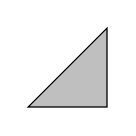
\begin{tikzpicture}
        \filldraw[fill=lightgray] (0,0) -- (0:1) -- ++(90:1) -- cycle;
    \end{tikzpicture}

    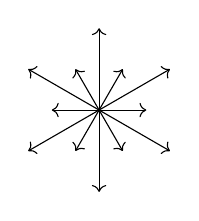
\begin{tikzpicture}
        \draw[->] (0,0) -- (0:0.6);
        \draw[->] (0,0) -- ($ (0:0.6) + (60:0.6) $);
        \draw[->] (0,0) -- (60:0.6);
        \draw[->] (0,0) -- ($ (60:0.6) + (120:0.6) $);
        \draw[->] (0,0) -- (120:0.6);
        \draw[->] (0,0) -- ($ (120:0.6) + (180:0.6) $);
        \draw[->] (0,0) -- (180:0.6);
        \draw[->] (0,0) -- ($ (180:0.6) + (240:0.6) $);
        \draw[->] (0,0) -- (240:0.6);
        \draw[->] (0,0) -- ($ (240:0.6) + (300:0.6) $);
        \draw[->] (0,0) -- (300:0.6);
        \draw[->] (0,0) -- ($ (300:0.6) + (0:0.6) $);
    \end{tikzpicture}
    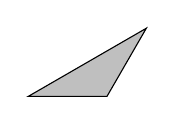
\begin{tikzpicture}
        \filldraw[fill=lightgray] (0,0) -- (0:1) -- ++(60:1) -- cycle;
    \end{tikzpicture}
    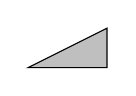
\begin{tikzpicture}
        \filldraw[fill=lightgray] (0,0) -- (0:1) -- ++(90:0.5) -- cycle;
    \end{tikzpicture}
\end{frame}

\begin{frame}
    \frametitle{空間の敷き詰め}

    この対応関係は2次元だけでなく、より高い次元でも成り立ちます。

    \bigskip

    \begin{block}{問題}
        三角錐を面で折り返す(鏡映)操作を繰り返すとき、
        互いに重ならずに、すき間なく空間を埋め尽くすことができる条件は?
    \end{block}

    3次元のルート系は、\(A_3\), \(B_3\), \(C_3\) があります。
    このそれぞれについて、3次元空間を埋め尽くす三角錐が対応しており、
    上記の問題の解はその3通りです。

    \bigskip

    4次元以上でも同様です。単体(三角形や三角錐)を超平面で鏡映する操作を繰り返すとき、
    互いに重ならずに、すき間なく空間を埋め尽くすことができるものは、
    その次元のルート系と対応しています。
\end{frame}

\begin{frame}
    \frametitle{参考文献}

    \begin{itemize}
        \item 松澤淳一、特異点とルート系、朝倉書店(すうがくの風景シリーズ6)
        \item 松澤淳一、数学セミナー2009年10月号 ディンキン図形とルート系、日本評論社
    \end{itemize}
\end{frame}

\end{document}
